\chapter{Implementation structure}
Implementation chapter reveals the overall application architecture overview. Its purpose is to provide the information using which the experienced developer can understand and further improve the project. 

At first, we summarize the overall solution design. Then we go through the project file structure and describe the application architecture and structure. In the end, we focus on the implementation details of some of the application parts and emphasize the things that are not obvious from the project structure and conventions.


\section{Project architecture}
schema services \todo {services schema}

\begin{figure}[h]\centering
	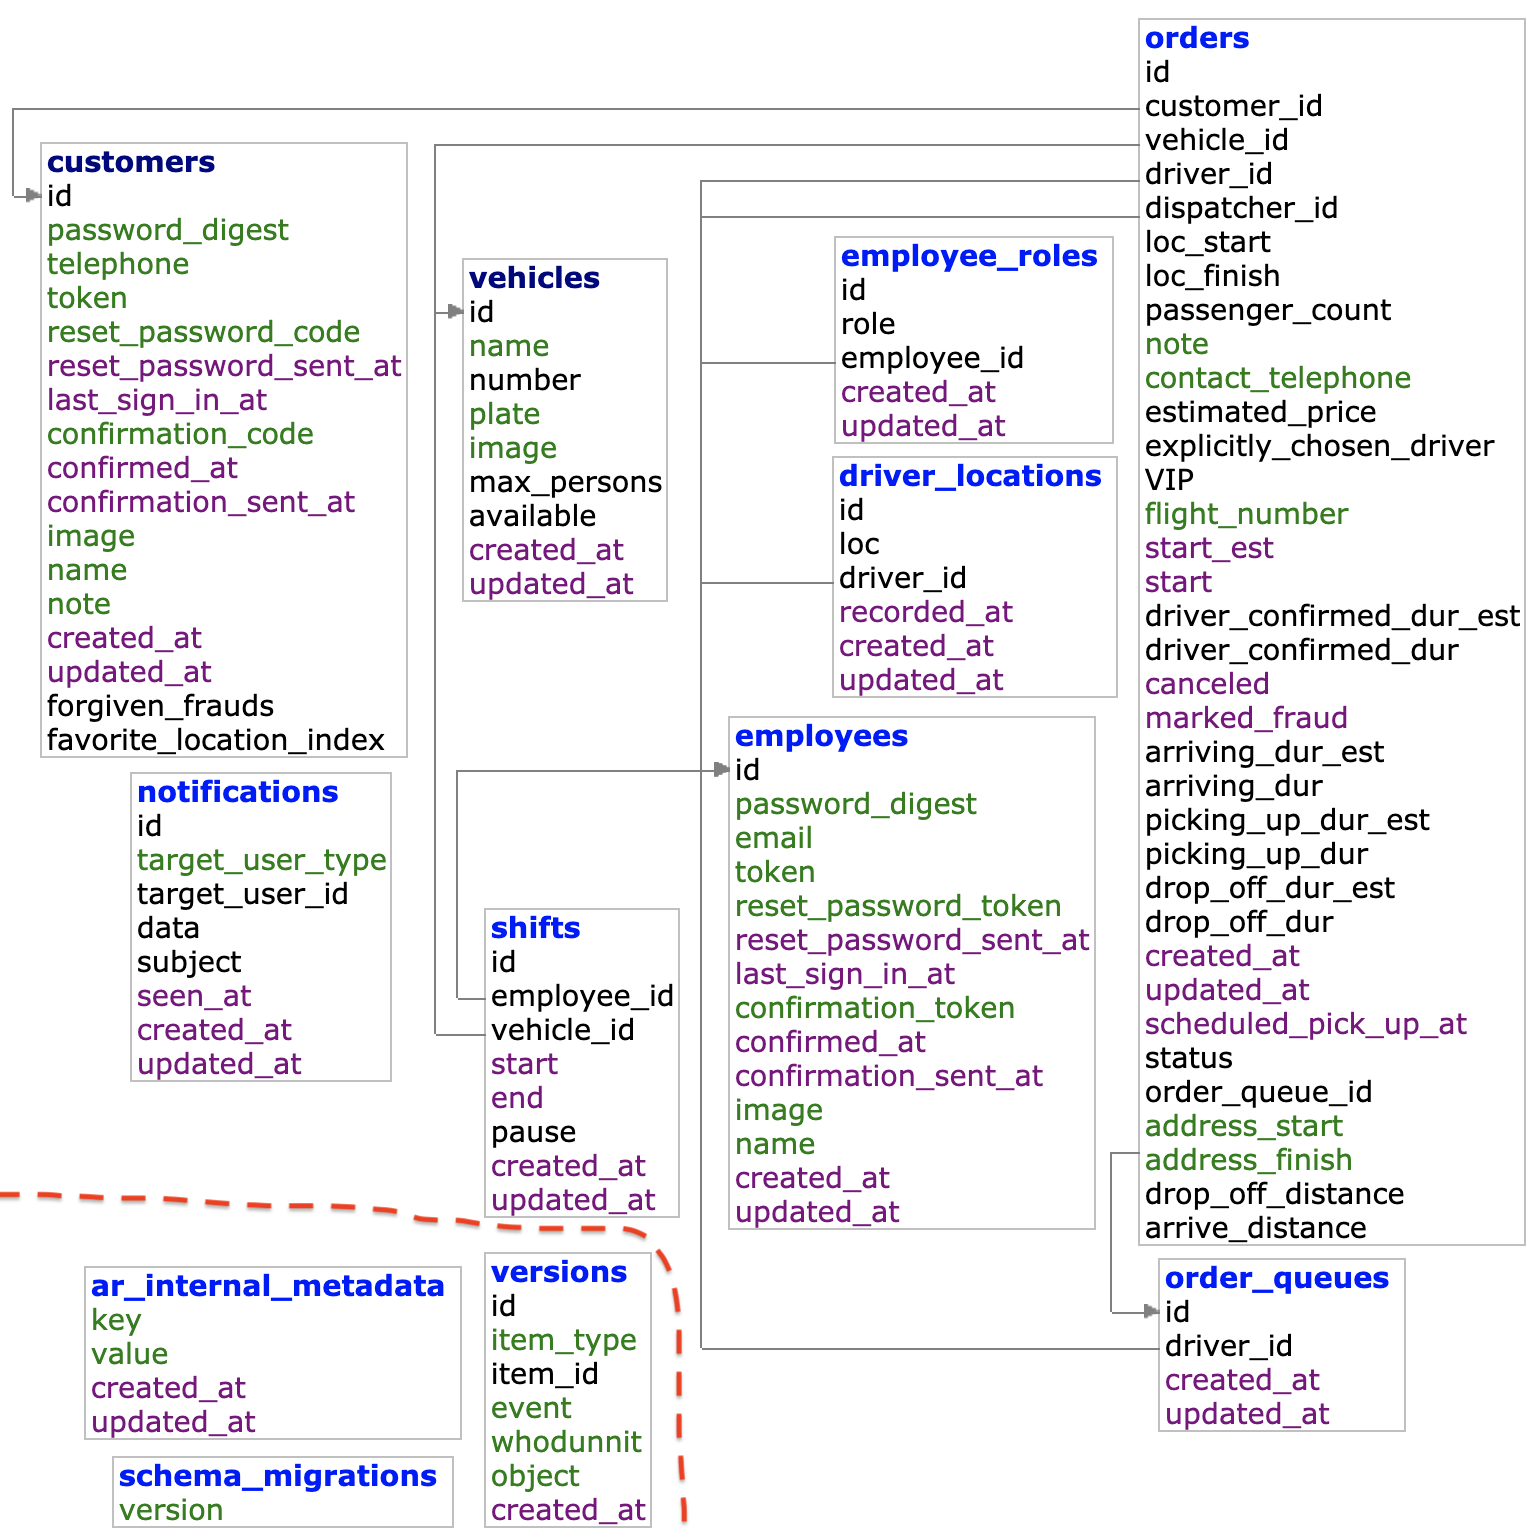
\includegraphics[scale=0.53]{db_schema.png}
	\caption{Database schema} 
	\label{database-schema}
\end{figure} 


\section {Application file structure}
	Ruby on Rails is MVC framework. We suppose, that the reader is familiar with the MVC\footnote{\url{https://en.wikipedia.org/wiki/Model\%E2\%80\%93view\%E2\%80\%93controller}} pattern.
	
	Ruby on Rails framework is tightly connected with the Convention over configuration software design paradigm. In short that means that we as a programmer are forced to use Rails conventions otherwise it will not work. This implies that the whole project file structure or class naming conventions are strictly given. 
	
	We followed these conventions and tools that the framework gives us as best as we can. In this section we are going to describe them and the way how we approached them within our application.
	
	Whole Rails application lays in \textit{TaxiBackendApp} folder. In this section we describe all of the key files and folders that we  use in our project. All the other files and folders which are not described in this section can be ignored - they are either automatically generated by the framework or we didn't needed that feature of the framework during the development.
	
	These are the key folders and files in our project: 
	\begin{itemize}
		\item app
			\begin{itemize}
				\item controllers
				\item helpers
				\item lib
				\item mailers
				\item models
				\item policies
				\item uploaders
				\item validators
				\item views
				\item workers
			\end{itemize}
		\item config \begin{itemize}
			\item environments
			\item initializers
			\item locales
			\item database.yml
			\item routes.rb
			\item sidekiq.yml
		\end{itemize}
		\item db \begin{itemize}
			\item migrate
			\item seeds.rb
			\item schema.rb
		\end{itemize}
		\item lib
		\item public
		\item spec \begin{itemize}
			\item factories
			\item requests
		\end{itemize}
		\item Gemfile
	\end{itemize}

	\subsection{app/controllers}
		In this folder are placed all the controllers we use in the application. All of the controllers in Ruby on Rails must inherit from the \textit{ApplicationController}. Because we are writing API which may have next versions in the future, we decided to add one more layer - \textit{ApiV2Controller} which takes care about the API-specific general tasks such as authorization. This implies that all the controllers for our API are inherited from this controller.
		
		Each controller is separate file in which is just one - the controller class.
		
		Each public method in the controller class is considered as action which can be binded to the router. Default actions are:
		\begin{itemize}
			\item index = display all entities
			\item show = show specific entity
			\item create
			\item update
			\item destroy		
		\end{itemize} 
	
		Best practice is to fit with most of the actions on the entities in these names. For action show, update and destroy we suppose that we get entity id from the router.
	\subsection{app/helpers}
		This folder contains helpers for the application. Helpers are specific functions which are more general for the application and we want to have them separated for better code readability. 
		
		In our application was the helpers folder the first choice where to put the calculation of the distance between the two coordinates, because we use it in both controllers and workers and it is quite complex function to have it directly in place.
	\subsection{app/lib}
		This folder is usually the folder where you place everything which can not be classified to one of the default Ruby on Rails framework predefined folders. Usually it is the code containing custom logic related to the problem the application is solving.
		
		In our case this folder contains whole orders scheduler including the Google Matrix API wrapper.
		
	\subsection{app/mailers}
		Ruby on Rails has built-in support for sending emails. For each entity we can create class called Mailer, which can have multiple methods - specific emails and its configurations, based on which the email is later sent. Using this mailer provides us out-of-the box asynchronous queue sending via SMTP - configured in \textit{config/initializers} folder.
		 
		 The mail template which will be used for the email is specified in the \textit{views/entity\_mailer/action\_mail.*}.
		 
		 In our application we used these mailers for the employees registration and forgotten password mails.
	\subsection{app/models}
		Models folder contains all the application models. Ruby on Rails provide rich ORM library called ActiveRecord, which is the implementation of the same named design pattern\footnote{\url{https://en.wikipedia.org/wiki/Active\_record\_pattern}}.
		
		In our application each of the model classes corresponds to one database table. In the model classes we also define relations between the models and validations of the model attributes. 
		
		In the models folder there is folder called \textit{concerns}. This folder contains separated logic which is used by more models. In our application we use the concerns for authentication, user roles and notification - all of them are used by the Customer and Employee model, thus it is convenient to have it separated at a separate place.
		
		Another interesting pattern we use a lot in our application are model scopes. Scopes allows us to have defined commonly used filters or queries directly on the model class. For example we have scope \textit{dispatchers} for the \textit{Employee} model, which selects dispatchers only from the set of employees.
		
	\subsection{app/policies}
		Policies folder is the place where we have all the permission definitions which uses the Pundit gem. Basic principles how the policy definition works and how it is connected with the rest of the application is described later in the \ref{implementation_authorization} 
	\subsection{app/uploaders}
		Here lies the configuration file for our \textit{Carierwave} uploader used for images of the employees and vehicles. 
	\subsection{app/validators}
		During the creation of the order model we end up with the complicated validator definition. For the better code readability we decide separate that validator to custom file, which lies in this folder. 
		
		Even though the orders validator is the only one such complicated that we felt the urge to separate it to its own file, this folder can be used in the future for other complicated validators in the application.
		  
	\subsection{app/views}
		In this folder is the view part of the application.  In the \textit{employee\_mailer} folder we can find templates for the emails. Inside the \textit{api/v2} we have the Jbuilder templates for our endpoints. \textit{Index.*} is usually for showing collection of specified items, \textit{show.*} is for displaying one specific item. Files starting with underscore are called partials. Partials are separated parts of views which are used on more places across the views.
	\subsection{app/workers}
		In the workers folder lies all the Sidekiq workers. In general we can say that if there is some code running asynchronously in our application, it is in this folder. 
	\subsection{config/environments}
		Here lies the configuration files specific for the development, testing and production environment. Especially we can find there mail and logs configurations. 
	\subsection{config/initializers}
		Ruby on Rails has special folder for initialization and configuration of the modules and classes used in the application. Especially there are initializers for Google Maps API, Sidekiq (asynchronous jobs), Kaminari (pagination), Lograge (logs formatting), CML (our order scheduler) and CORS.
	\subsection{config/locales}
		Inside this folder we have for each language one YAML file which defines translations for the whole application.dss
	\subsection{config/database.yml}
		Database YAML file define which database we use on which environment and specifies how to connect to database server and which database use there.
	\subsection{config/routes.rb}
		Inside routes file we define all our API endpoints. Ruby on Rails has actions index, show, create, update and destroy on each entity by default. It requires for each resource having controller of the same name, where are the actions defined as methods.
	\subsection{config/sidekiq.yml}
		Inside the sidekiq configuration file we can set thread count which will the job processor run on and also job queue names - in our case mailers and default queue which is processing everything except the mails.
	\subsection{db/migrate}
		Whole database is created and modified through migrations. Each of these migrations is described in its specific file. Some of them are generated via Rails CLI.
	\subsection{db/seeds.rb}
		Inside seeds file are defined initial data which are inserted to the database when the \textit{rake db:seed} command is called. In our application we use it for setting up the initial administrator account.
	\subsection{db/schema.rb}
		This file is automatically generated by the Ruby on Rails from the migrations. It contains whole database schema with the table columns properties and table indexes.
	\subsection{lib}
		This folder contains in our application only custom Rake task definitions. In our case the generator tasks for generating mock data.
	\subsection{public}
		Public folder is for the application static assets. Especially this is the place where all the vehicle and employee images are located.
	\subsection{spec/factories}
		For the mocks generation in our tests we use FactoryBot\footnote{\url{https://github.com/thoughtbot/factory_bot}} gem. Factories folder holds definitions of these factories from which mocks are created.
	\subsection{spec/requests}
		The only tests we have written as part of the thesis are in this folder. Each entity has its own file inside which are the tests structured using the \textit{Context} and \textit{Describe} blocks.
	\subsection{Gemfile}
		Gemfile specifies library (gem) project dependencies. Each gem record also contains version described based on which the libraries can be automatically updated. This file is similar to the \textit{package.json} file in javascript NPM projects.
\section {Specific implementation details}
\subsection {Authentication}
We created concern \textit{AuthenticableUser} which is included in both Customer and Employees model. The concern takes care of auth token generation and manipulation using \textit{has\_secure\_token} \footnote{\url{https://api.rubyonrails.org/classes/ActiveRecord/SecureToken/ClassMethods.html}} Rails utility. 

\textit{ApiV2Controller} is the one responsible for checking auth token in headers and setting the current user variable for all the controllers.

SMS workers now just print tokens to logs. When we go to production we just sent this token to some third-party SMS gateway API.

Mailer used for employees token sending is not connected to mail server. All the mails now goes Mailtrap\footnote{\url{https://mailtrap.io/}}, which is a fake SMTP server. In production we must switch to real one. Once we have them, just change the \textit{config/environments/production.rb} config.action\_mailer section

\label{implementation_authorization}\subsection {Authorization}
We use \textit{Pundit} gem to help us with authorization. For each controller in \textit{api/v2} there is one permissions definition file in \textit{politions} folder with the according name.  This file contains policy class. 

Each method in this policy class is permission definition for the corresponding action in controller. There could also be scope definitions. Their purpose is to return subset of the current entities to which has current user access to. Last type of methods that can appear in these files are custom policy definition methods. These methods check other specific actions needed somewhere in the application and they are called explicitly from views or controllers.

The whole Pundit initialization is in \textit{api/v2/api\_v2\_controller.rb} where is also defined what the application should do if the request is unauthorized. As we can see, our implementation returns error 403 with 'not authorized' error as specified.

In each controller action we must call the \textit{authorize} method which will automatically checks the permissions for us. If we don't want to authorize the request we must explicitly call \textit{skip\_authorization}. In case we don't call it, there will be raised missing authorization exception on such endpoint. This mechanism is there to prevent the situation when programmer forgets to set authorization for the endpoint, which would lead to possible sensitive data exposure.

\subsection{Order scheduler}
\todo{dopsat}
\subsection{Favorite locations}
\todo{dopsat}
\subsection{Generators}
\todo{dopsat}